% !TeX program = xelatex
% Build from the project root with build.ps1 -Document exercises/5/main.tex.
\documentclass[12pt,a4paper]{article}
\RequirePackage{array}[=2024-06-01]
% !TeX root = ../2/main.tex
\usepackage[a4paper,margin=25mm,headheight=16pt]{geometry}
\usepackage{amsmath,amssymb}
\usepackage{graphicx}
\usepackage{booktabs}
\usepackage{tabularx}
\usepackage{siunitx}
\usepackage{tikz}
\usepackage{circuitikz}
\usepackage[unicode,hidelinks]{hyperref}
\usepackage{xepersian}
% Only the regular B Nazanin file is installed; synthesize bold explicitly.
\settextfont[Path=C:/Windows/Fonts/,AutoFakeBold=2,AutoFakeSlant=0.2]{B-NAZANIN.TTF}
% B Nazanin lacks U+066A (Arabic percent), required by xepersian's digit setup.
% Arial covers the complete required digit/punctuation set; Persian prose remains B Nazanin.
\setdigitfont[Path=C:/Windows/Fonts/,BoldFont=arialbd.ttf,ItalicFont=ariali.ttf,BoldItalicFont=arialbi.ttf]{arial.ttf}
\setmathdigitfont[Path=C:/Windows/Fonts/,BoldFont=arialbd.ttf,ItalicFont=ariali.ttf,BoldItalicFont=arialbi.ttf]{arial.ttf}
\setlatintextfont{TeX Gyre Termes}
% B Nazanin does not contain the default itemize bullet and dash glyphs.
\renewcommand{\labelitemi}{\(\bullet\)}
\renewcommand{\labelitemii}{\(\circ\)}
\renewcommand{\labelitemiii}{\(\diamond\)}
\setlength{\parindent}{0pt}
\setlength{\parskip}{0.5em}
\linespread{1.25}
\newcommand{\exercise}[1]{\section*{تمرین #1}}
% !TeX root = ../2/main.tex
% Shared title page for every assignment.
% Change only \AssignmentNumber and \AssignmentDate in each main document.

\newcommand{\AssignmentNumber}[1]{\gdef\assignmentnumber{#1}}
\newcommand{\AssignmentDate}[1]{\gdef\assignmentdate{#1}}

\newcommand{\assignmentnumber}{---}
\newcommand{\assignmentdate}{---}

% Stable course metadata
\newcommand{\universityname}{دانشگاه صنعتی امیرکبیر}
\newcommand{\universityalias}{پلی‌تکنیک تهران}
\newcommand{\facultyname}{دانشکده مهندسی کامپیوتر}
\newcommand{\coursename}{طراحی مدارهای مجتمع پرتراکم پیشرفته}
\newcommand{\studentname}{محمد خلیلی اصل}
\newcommand{\instructorname}{دکتر مهدی صدیقی}

\newcommand{\MakeAssignmentCover}{%
  \begin{titlepage}
    \thispagestyle{empty}
    \centering
    \linespread{1}\selectfont

    \vspace*{0mm}
    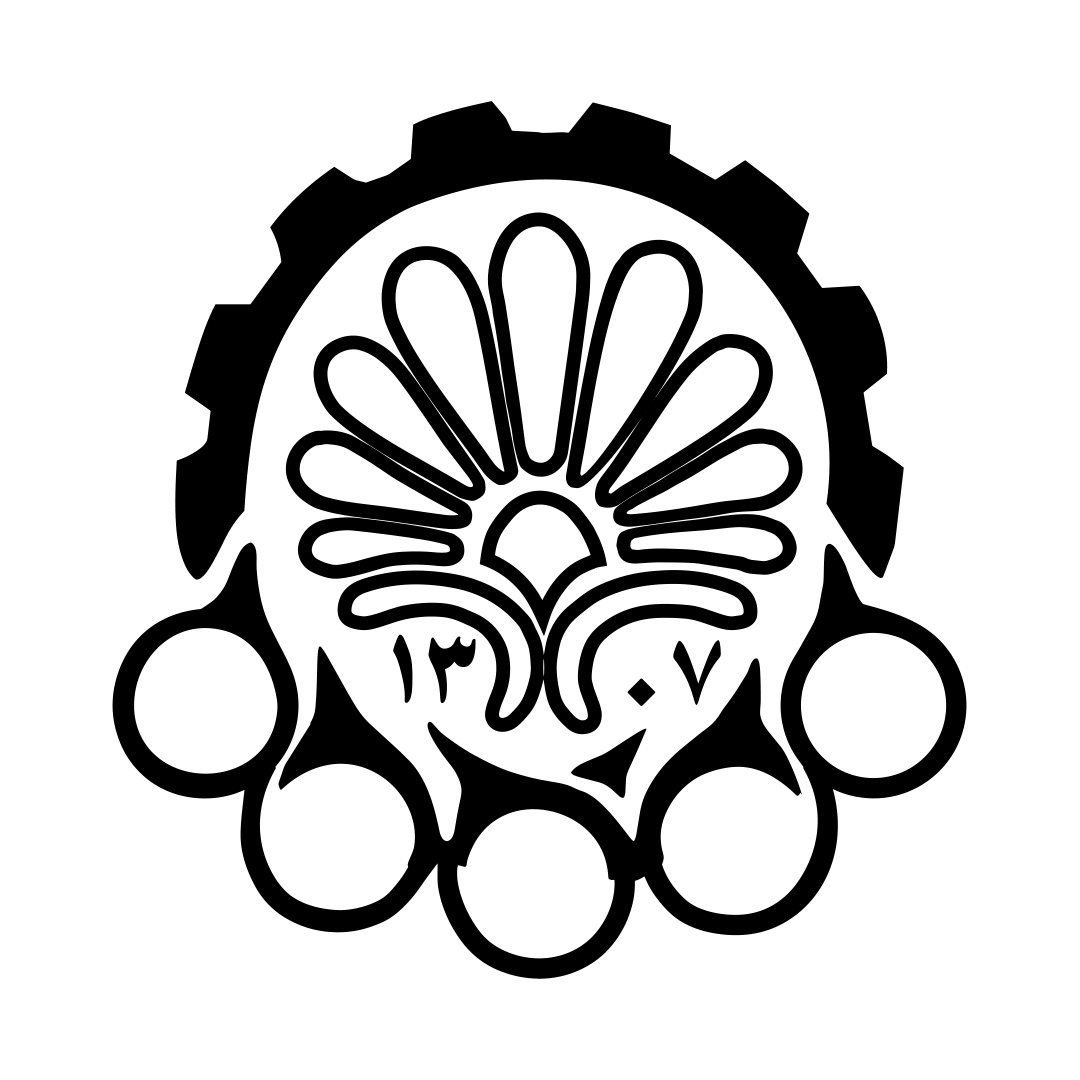
\includegraphics[width=44mm]{assets/aut-logo-black.png}\par
    \vspace{3mm}

    {\Large\bfseries \universityname\par}
    \vspace{1mm}
    {\large (\universityalias)\par}
    \vspace{1mm}
    {\large \facultyname\par}

    \vspace{8mm}
    {\Large\bfseries درس \coursename\par}

    \vspace{12mm}
    {\large عنوان\par}
    \vspace{2mm}
    {\LARGE\bfseries تمرین شماره \assignmentnumber\par}

    \vspace{10mm}
    {\large تهیه‌کننده\par}
    \vspace{2mm}
    {\Large\bfseries \studentname\par}

    \vspace{10mm}
    {\large استاد درس\par}
    \vspace{2mm}
    {\Large\bfseries \instructorname\par}

    \vspace{10mm}
    {\Large \assignmentdate\par}
    \vfill
  \end{titlepage}
  \setcounter{page}{1}%
}


% Shared bibliographic text. Coverage notes remain in each booklet.
\newcommand{\WesteReference}{%
\begin{latin}
Neil H. E. Weste and David Money Harris,
\textit{CMOS VLSI Design: A Circuits and Systems Perspective},
Fourth Edition, Addison-Wesley (Pearson Education), 2011.
\end{latin}%
}

\XeTeXgenerateactualtext=1
\newcommand{\secnum}[1]{\texorpdfstring{\mbox{\beginL#1\endL}}{#1}}
% The headings display the original textbook exercise numbers.
\setcounter{secnumdepth}{0}
\setlength{\emergencystretch}{3em}
\AtBeginDocument{\DeclareSIPrefix{\micro}{\text{\lr{µ}}}{-6}}
\hypersetup{pdftitle={تمرینات فصل ۵},pdfauthor={محمد خلیلی اصل}}
\AssignmentNumber{تمرینات فصل ۵}
\AssignmentDate{}
\patchcmd{\MakeAssignmentCover}{تمرین شماره \assignmentnumber}{\assignmentnumber}{}{\errmessage{Cover title replacement failed}}

\begin{document}
\MakeAssignmentCover
\section{حل تمرین‌های \lr{Power}}
\label{sec:power-assignment}

تمرین‌های این مجموعه در اسلاید ۲۴ درس مشخص شده‌اند. صورت‌ها از فصل
\lr{Power} کتاب بازنویسی شده‌اند. در قرارداد کتاب، \lr{Activity Factor}
میانگین تعداد گذارهای صعودی در هر دوره ساعت است. فرض‌های مربوط به
استقلال ورودی‌ها و مدل افت تغذیه در حل هر تمرین آمده‌اند
\cite[تمرین‌های فصل ۵، صفحات ۲۰۹ و ۲۱۰]{weste}
\cite[اسلاید ۲۴]{powerslides}.

% !TeX root = ../main.tex
\subsection{تمرین \secnum{۵.۱}، تخمین توان سوئیچینگ تراشه}
\label{sec:assignment-power-chip}

\textbf{خواسته.}
تراشه‌ای از منطق تصادفی با \lr{Activity Factor} متوسط \(\alpha=0.1\)
در نظر بگیرید. ظرفیت سوئیچینگ بر واحد سطح در فرایند \lr{Standard Cell}
برابر \(c_A=\qty[per-mode=symbol]{450}{\pico\farad\per\square\milli\metre}\)
است. با مساحت \(A=\qty{70}{\square\milli\metre}\)، فرکانس
\(f=\qty{450}{\mega\hertz}\) و تغذیه \(V_{DD}=\qty{0.9}{\volt}\)،
توان دینامیکی تراشه را تخمین بزنید \cite[تمرین \secnum{۵.۱}، صفحه ۲۰۹]{weste}.

\textbf{حل.}
چگالی ظرفیت را در مساحت ضرب می‌کنیم تا ظرفیت کلِ پیش از وزن‌دهی
با فعالیت، یعنی \(C\)، به دست آید. واحد مساحت در ضرب ساده می‌شود.
\[
  C=c_AA=\qty{31500}{\pico\farad}=\qty{31.5}{\nano\farad}.
\]
برای اعمال فعالیت متوسط بر کل ظرفیت، مقدار \(0.1\) را نماینده
میانگین وزن‌دار \(\alpha=\sum_i\alpha_i C_i/\sum_i C_i\) می‌گیریم
که \(C_i\) و \(\alpha_i\) ظرفیت و فعالیت گره \(i\) هستند.
پس ظرفیت مؤثر \(\alpha C\) است. با فرض ناچیز بودن جریان
مستقیمِ گذرا، توان دینامیکی را با توان سوئیچینگ برآورد می‌کنیم
\cite[رابطه \secnum{۵.۱۰}، صفحه ۱۸۴]{weste}.
\[
  \begin{aligned}
    P_{\mathrm{dyn}}&\approx \alpha C V_{DD}^{2} f\\
      &=0.1(\qty{31.5e-9}{\farad})(\qty{0.9}{\volt})^{2}
             (\qty{450e6}{\hertz})\approx\qty{1.15}{\watt}.
  \end{aligned}
\]
حاصل ضرب فاراد و مربع ولت، ژول است. ضرب در هرتز آن را به وات
تبدیل می‌کند. مقدار نمایش‌داده‌شده به دو رقم اعشار گرد شده و
برآورد در مرتبه‌ی یک وات است.

% !TeX root = ../main.tex
\subsection{تمرین \secnum{۵.۴}، فعالیت از روی شکل موج}
\label{sec:assignment-power-waveform}

\textbf{خواسته.}
برای سیگنال شکل \secnum{۵.۳۴} کتاب با ساعت \qty{1}{\giga\hertz}،
\lr{Activity Factor} را تعیین کنید. شکل \ref{fig:assignment-power-waveform}
بازه و لبه‌های صعودی را نشان می‌دهد
\cite[تمرین \secnum{۵.۴}، صفحه ۲۰۹]{weste}.

\begin{figure}[htbp]
  \centering
  % Shared redraw of the exercise waveform for the notes and submission.
\begin{latin}
\begin{tikzpicture}[x=1.08cm,y=1.30cm]
  \draw[->] (0,-0.30) -- (10.75,-0.30) node[right] {\(t\,(\unit{\nano\second})\)};
  \node[left] at (-0.08,1.24) {\(v/V_{DD}\)};
  \node[left] at (-0.08,0) {\rl{۰}};
  \node[left] at (-0.08,1) {\rl{۱}};
  \foreach \x/\ticklabel in {0/۰,1/۱,2/۲,3/۳,4/۴,5/۵,6/۶,7/۷,8/۸,9/۹,10/۱۰} {
    \draw (\x,-0.25) -- (\x,-0.36) node[below] {\rl{\ticklabel}};
  }
  \draw[gray,densely dashed] (1,-0.24) -- (1,0.50);
  \draw[gray,densely dashed] (4,-0.24) -- (4,0.50);
  \draw[very thick] (0,0) -- (0.75,0) -- (1.25,1) -- (1.75,1)
    -- (2.25,0) -- (3.75,0) -- (4.25,1) -- (7.75,1) -- (8.25,0) -- (10,0);
  \fill (1,0.50) circle (1.5pt) (4,0.50) circle (1.5pt);
\end{tikzpicture}
\end{latin}

  \caption{بازرسم شکل \secnum{۵.۳۴} کتاب با محور ولتاژ نرمال‌شده.
    نقطه‌ها دو گذار صعودی در بازه مشاهده را مشخص می‌کنند \cite{weste}.}
  \label{fig:assignment-power-waveform}
\end{figure}

\textbf{حل.}
دوره ساعت \(T_{\mathrm{clk}}=1/f=\qty{1}{\nano\second}\) است.
در فاصله‌ی صفر تا \qty{10}{\nano\second}، ده دوره کامل داریم.
خروجی نزدیک \qty{1}{\nano\second} و \qty{4}{\nano\second} از
صفر به یک می‌رود. شمار گذار صعودی \(N_{\uparrow}=2\) و شمار
دوره ساعت \(N_{\mathrm{clk}}=10\) است. بر اساس تعریف کتاب، حاصل چنین است
\cite[بخش \secnum{۵.۱.۲}، صفحه ۱۸۴]{weste}.
\[
  \alpha=\frac{N_{\uparrow}}{N_{\mathrm{clk}}}=\frac{2}{10}=0.2.
\]
در قرارداد این فصل، هر گذار صعودی یک رویداد شارژ است و شارژها
در صورت کسر شمرده می‌شوند.

% !TeX root = ../main.tex
\subsection{تمرین \secnum{۵.۷}، استخراج احتمال‌های گیت‌ها}
\label{sec:assignment-power-probability}

\textbf{خواسته.}
احتمال‌های جدول \secnum{۵.۱} کتاب را از تابع منطقی هر گیت به دست
آورید \cite[جدول \secnum{۵.۱}، صفحه ۱۸۷ و تمرین \secnum{۵.۷}،
صفحه ۲۰۹]{weste}.

\textbf{حل.}
برای سیگنال \(X\)، \(p_X=\Pr(X=1)\) و
\(\bar p_X=1-p_X=\Pr(X=0)\) را تعریف می‌کنیم. فرض می‌کنیم
ورودی‌ها در یک دوره مستقل‌اند، پس احتمال یک ترکیب ورودی از ضرب
احتمال‌های آن به دست می‌آید. \(Y\) خروجی گیت است.

\begin{itemize}
  \item \lr{AND2} فقط در حالت \((1,1)\) خروجی یک دارد، پس
    \(p_Y=p_Ap_B\). \lr{AND3} فقط در حالت \((1,1,1)\)
    خروجی یک دارد، پس \(p_Y=p_Ap_Bp_C\).
  \item \lr{NOR2} فقط با دو ورودی صفر خروجی یک دارد، بنابراین
    \(p_Y=\bar p_A\bar p_B\). \lr{OR2} خروجی آن را معکوس می‌کند،
    پس \(p_Y=1-\bar p_A\bar p_B\) است.
  \item \lr{NAND2} مکمل \lr{AND2} است و \(p_Y=1-p_Ap_B\).
  \item \lr{XOR2} وقتی ورودی‌ها متفاوت‌اند خروجی یک دارد. دو
    حالت \((1,0)\) و \((0,1)\) هم‌زمان رخ نمی‌دهند، پس
    احتمال‌هایشان با هم جمع می‌شوند و
    \(p_Y=p_A\bar p_B+\bar p_Ap_B\) به دست می‌آید.
\end{itemize}

ستون احتمال جدول کتاب با این روابط به دست می‌آید. اگر علاوه‌بر
استقلال ورودی‌ها در هر دوره، بردار ورودی در دوره‌های متوالی مستقل
و هم‌توزیع باشد و بین نمونه‌ها گذار اضافی رخ ندهد، احتمال گذار
صعودی خروجی از ضرب احتمال صفر در دوره فعلی و احتمال یک در دوره
بعد به دست می‌آید \cite[رابطه \secnum{۵.۱۴}، صفحه ۱۸۷]{weste}.
\[
  \alpha_Y=\Pr(Y_k=0,Y_{k+1}=1)
          =(1-p_Y)p_Y.
\]
\(Y_k\) مقدار خروجی در دوره \(k\) است. به‌عنوان کنترل، با فرض
احتمال \(1/2\) برای هر ورودی، نتیجه گیت‌ها به ترتیب جدول
\ref{tab:assignment-power-probabilities} است.

\begin{table}[htbp]
  \centering
  \caption{احتمال یک‌بودن و \lr{Activity Factor} خروجی در حالت
    ورودی‌های مستقل و هم‌احتمال، با استقلال بین دوره‌ها. ستون رابطه
    از جدول \secnum{۵.۱} کتاب استخراج شده است \cite{weste}.}
  \label{tab:assignment-power-probabilities}
  \begin{tabular}{rccc}
    \toprule
    گیت & رابطه \(p_Y\) & \(p_Y\) در مثال & \(\alpha_Y\) در مثال \\
    \midrule
    \lr{AND2}  & \(p_Ap_B\) & \(1/4\) & \(3/16\) \\
    \lr{AND3}  & \(p_Ap_Bp_C\) & \(1/8\) & \(7/64\) \\
    \lr{OR2}   & \(1-\bar p_A\bar p_B\) & \(3/4\) & \(3/16\) \\
    \lr{NAND2} & \(1-p_Ap_B\) & \(3/4\) & \(3/16\) \\
    \lr{NOR2}  & \(\bar p_A\bar p_B\) & \(1/4\) & \(3/16\) \\
    \lr{XOR2}  & \(p_A\bar p_B+\bar p_Ap_B\) & \(1/2\) & \(1/4\) \\
    \bottomrule
  \end{tabular}
\end{table}

% !TeX root = ../main.tex
\subsection{تمرین \secnum{۵.۱۰}، اندازه‌گذاری \lr{pMOS Header}}
\label{sec:assignment-power-header}

\textbf{خواسته.}
در یک مدار \lr{Power Gating} با فرایند \qty{65}{\nano\metre}،
عرض کلید \lr{pMOS Header} را تعیین کنید تا افزایش تأخیر کمتر از
۲ درصد باشد. حاصل‌ضرب تقریبی مقاومت روشن کلید در عرض آن
\(r_w=\qty{2.5}{\kilo\ohm\micro\metre}\) و جریان فعال بلوک
\(I_{\mathrm{on}}=\qty{100}{\milli\ampere}\) است
\cite[تمرین \secnum{۵.۱۰}، صفحه ۲۱۰]{weste}.

\textbf{حل.}
با فرض تغذیه \(V_{DD}=\qty{1}{\volt}\) از مثال ۵.۵ کتاب،
از همان تقریب استفاده می‌کنیم که افزایش نسبی کوچک تأخیر را
با افت نسبی تغذیه برابر می‌گیرد. بنابراین در این مدل، برای
افزایش کمتر از ۲ درصد باید \(\Delta V<0.02V_{DD}=\qty{20}{\milli\volt}\)
باشد \cite[مثال ۵.۵، صفحات ۱۹۸ و ۱۹۹ و رابطه \secnum{۴.۲۹}،
صفحه ۱۶۲]{weste}.

با \(W\) به‌عنوان عرض مؤثر کلید و \(R_h\) به‌عنوان مقاومت روشن،
داریم \(R_h\approx r_w/W\) و \(\Delta V\approx I_{\mathrm{on}}R_h\).
در مدل مقاومتی، شرطِ افت به کران‌های زیر می‌انجامد.
\[
  \begin{aligned}
    R_h &< \frac{\qty{20}{\milli\volt}}{\qty{100}{\milli\ampere}}
          =\qty{0.20}{\ohm},\\
    W &> \frac{\qty{2.5e3}{\ohm\micro\metre}}{\qty{0.20}{\ohm}}
         =\qty{12.5e3}{\micro\metre}=\qty{12.5}{\milli\metre}.
  \end{aligned}
\]
عرض مرزی \qty{12.5}{\milli\metre} در این مدل متناظر با ۲ درصد
افزایش تأخیر است. شرطِ «کمتر از» عرضی بزرگ‌تر از این مرز می‌خواهد.
اگر کلید از چند ترانزیستور موازی ساخته شود، \(W\) مجموع عرض‌های
مؤثر است. برآورد عددی به فرض تغذیه، جریان نماینده و تقریب
افت ولتاژ در مثال کتاب وابسته است.


\clearpage
\begin{thebibliography}{9}
\bibitem{weste}
\WesteReference
فصل \lr{Power}، بخش‌های \secnum{۵.۱} تا \secnum{۵.۳} و تمرین‌ها،
به‌ویژه جدول \secnum{۵.۱}، مثال ۵.۵ و شکل \secnum{۵.۳۴}.
صورت تمرین‌ها در صفحات چاپی ۲۰۹ و ۲۱۰، برابر با صفحات ۲۳۶ و ۲۳۷
فایل \lr{PDF} است. مدل وابستگی تأخیر به تغذیه در بخش
\secnum{۴.۴.۶.۴}، صفحه چاپی ۱۶۲، معرفی شده است.
% !TeX root = ../complete.tex
\bibitem{powerslides}
\lr{Power}، از اسلایدهای \lr{CMOS VLSI Design, Fourth Edition}.
یادداشت‌های اصلی از \lr{David Money Harris} (۲۰۱۱) و توضیح
اقتباس در اسلاید ۲ مجموعه \lr{Introduction} آمده است.

\end{thebibliography}
\end{document}
